\documentclass{article}
\usepackage{CJK}
\usepackage{amsmath}
\usepackage{amsthm}
\usepackage{amsfonts}
\usepackage{palatino}
\usepackage{xcolor}
\usepackage{geometry}
\usepackage{listings}
\usepackage{pxfonts}
\usepackage{enumerate}
\usepackage[pdftex]{graphicx}
\geometry{left=2cm,right=2cm,top=3cm,bottom=3cm}
\pagestyle{myheadings}
\markright{Huiqian Yu/14300180118}
\setlength{\parindent}{0pt}
\newcommand{\ix}[1]{\intertext{{}#1}}
\newcommand{\dx}{\;\mathrm{d}\,x}
\newcommand{\dt}{\;\mathrm{d}\,t}
\newcommand{\dm}[1]{\;\mathrm{d}\,{}#1}
\newcommand{\ve}{\varepsilon}
\newcommand{\tp}{^\intercal}
\newcommand{\var}{\mathrm{var}}
\newcommand{\corr}{\mathrm{corr}}
\newcommand{\mbe}[1]{\mathbb{E}\left[{}#1\right]}
\newcommand{\argmin}[1]{\mathop{\arg\min}_{{}#1}}
\newcommand{\suml}[3]{\sum\limits_{#1=#2}^{#3}}
\newcommand{\e}{\mathrm{e}}
\newcommand{\vari}{\mathrm{i}}
\definecolor{backcolour}{rgb}{0.95,0.95,0.92}
\begin{document}
\begin{CJK*}{GBK}{song}

\section*{Problem 1}
Assume $X_2$ is $k$-dimensional,
\begin{align*}
f(X_1|X_2=x_2)&=\dfrac{f((X_1,X_2)\tp)}{f( X_2\tp)}\\
& = \frac{\sqrt{(2\pi)^k|\boldsymbol\Sigma_{22}|}\exp\left(-\frac 1 2 ((X_1,X_2)\tp-{\boldsymbol\mu})^\mathrm{T}{\boldsymbol\Sigma}^{-1}((X_1,X_2)\tp-{\boldsymbol\mu})\right)}{\sqrt{(2\pi)^d|\boldsymbol\Sigma|}\exp\left(-\frac 1 2 ( X_2\tp-{\boldsymbol\mu_2})^\mathrm{T}{\boldsymbol\Sigma_{22}}^{-1}(X_2\tp-{\boldsymbol\mu_2})\right)}
\ix{denote $X_1'=X_1-\mu_1, X_2'=X_2-\mu_2$,}\tag{M is a constant.}
& = M\exp{\left(-\frac 12 \left[(X_1',X_2')\Sigma^{-1}(X_1',X_2')\tp-X_2'\Sigma_{22}{}^{-1}X_2'{}^{\intercal}\right]\right)}
\ix{denote $\Sigma^{-1}=\left(\begin{array}{cc}
A&B\\
C&D
\end{array}\right)$, where $A$ is a $(d-k)\times(d-k)$ matrix.}
&=M\exp{\left(-\frac 12 \left[X_1'AX_1'{}^{\intercal}+X_1'BX_2'{}^{\intercal}+X_2'CX_1'{}^{\intercal}+X_2'DX_2'{}^{\intercal}\right]\right)}
\ix{since $\Sigma$ is symmetric, $B=C\tp$, assume $\mu'=BX_2'$,}\tag{E is a $k\times k$ matrix.}
&=M\exp{\left(-\frac 12 \left[(X_1'+\mu')A(X_1'+\mu')^{\intercal}-X_2'EX_2'{}^{\intercal}\right]\right)}\\
&=M\exp{\left(-\frac 12 (X_1-\mu_1+\mu')A(X_1-\mu_1+\mu')^{\intercal}\right)}
\end{align*}
This is a Multiple Normal Distribution with mean $\mu_1-\mu'$ and covariance $A^{-1}$.
\section*{Problem 2}
\begin{lstlisting}[language=R,keywordstyle=\color{blue!70},commentstyle=\color{red!50!green!50!blue!50},frame=single,rulesepcolor=\color{red!20!green!20!blue!20},backgroundcolor=\color{backcolour},
]
library(MASS)
x = seq(-5,5,0.02)
ker2 <- function(x,y){
  exp(-(abs(x-y)^2/2))
}
ker1 <- function(x,y){
  exp(-(abs(x-y)/2))
}
covMat <- function(x, kerFun){
  toReturn = matrix(rep(x, length(x)), length(x), length(x))
  apply(toReturn, 1, kerFun, y=x)
}
tshw9Plot <- function(isKer2 = T){
  if (isKer2) {
    kerFun = ker2
    main = 'Kernel with exponential 2'
  }else{
    kerFun = ker1
    main = 'Kernel with exponential 1'
  }
  y = mvrnorm(5, mu = rep(0, length(x)), Sigma = covMat(x, kerFun))
  for (i in 1:5){
    plot(x, y[i,], xlim=c(-5, 5), ylim = c(-5,5), lty = i, ylab='',
main=main, type = 'l')
    par(new = T)
  }
}
tshw9Plot(T)
par(new = F)
tshw9Plot(F)
\end{lstlisting}
The kernel function with exponential 2 is much more smoother.
\begin{center}
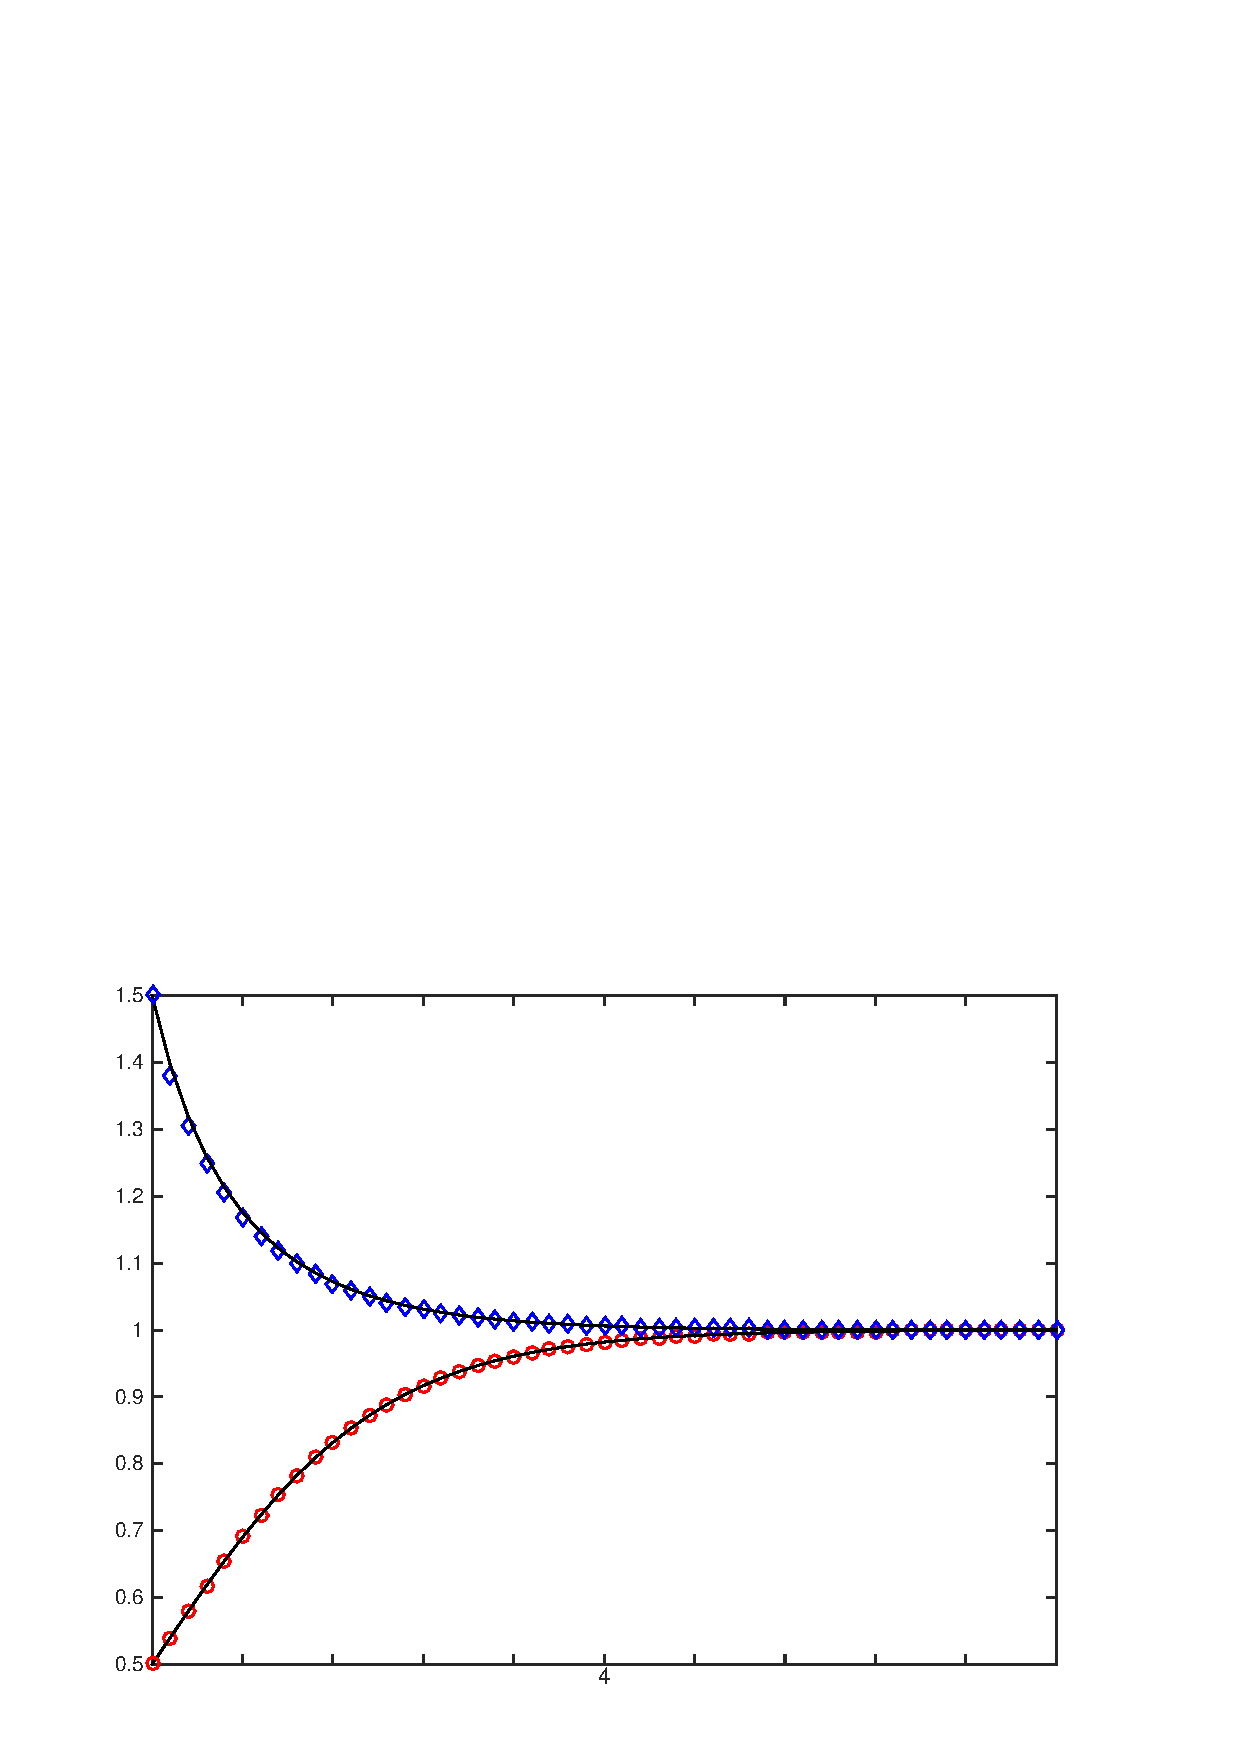
\includegraphics[width=8cm]{3.png}
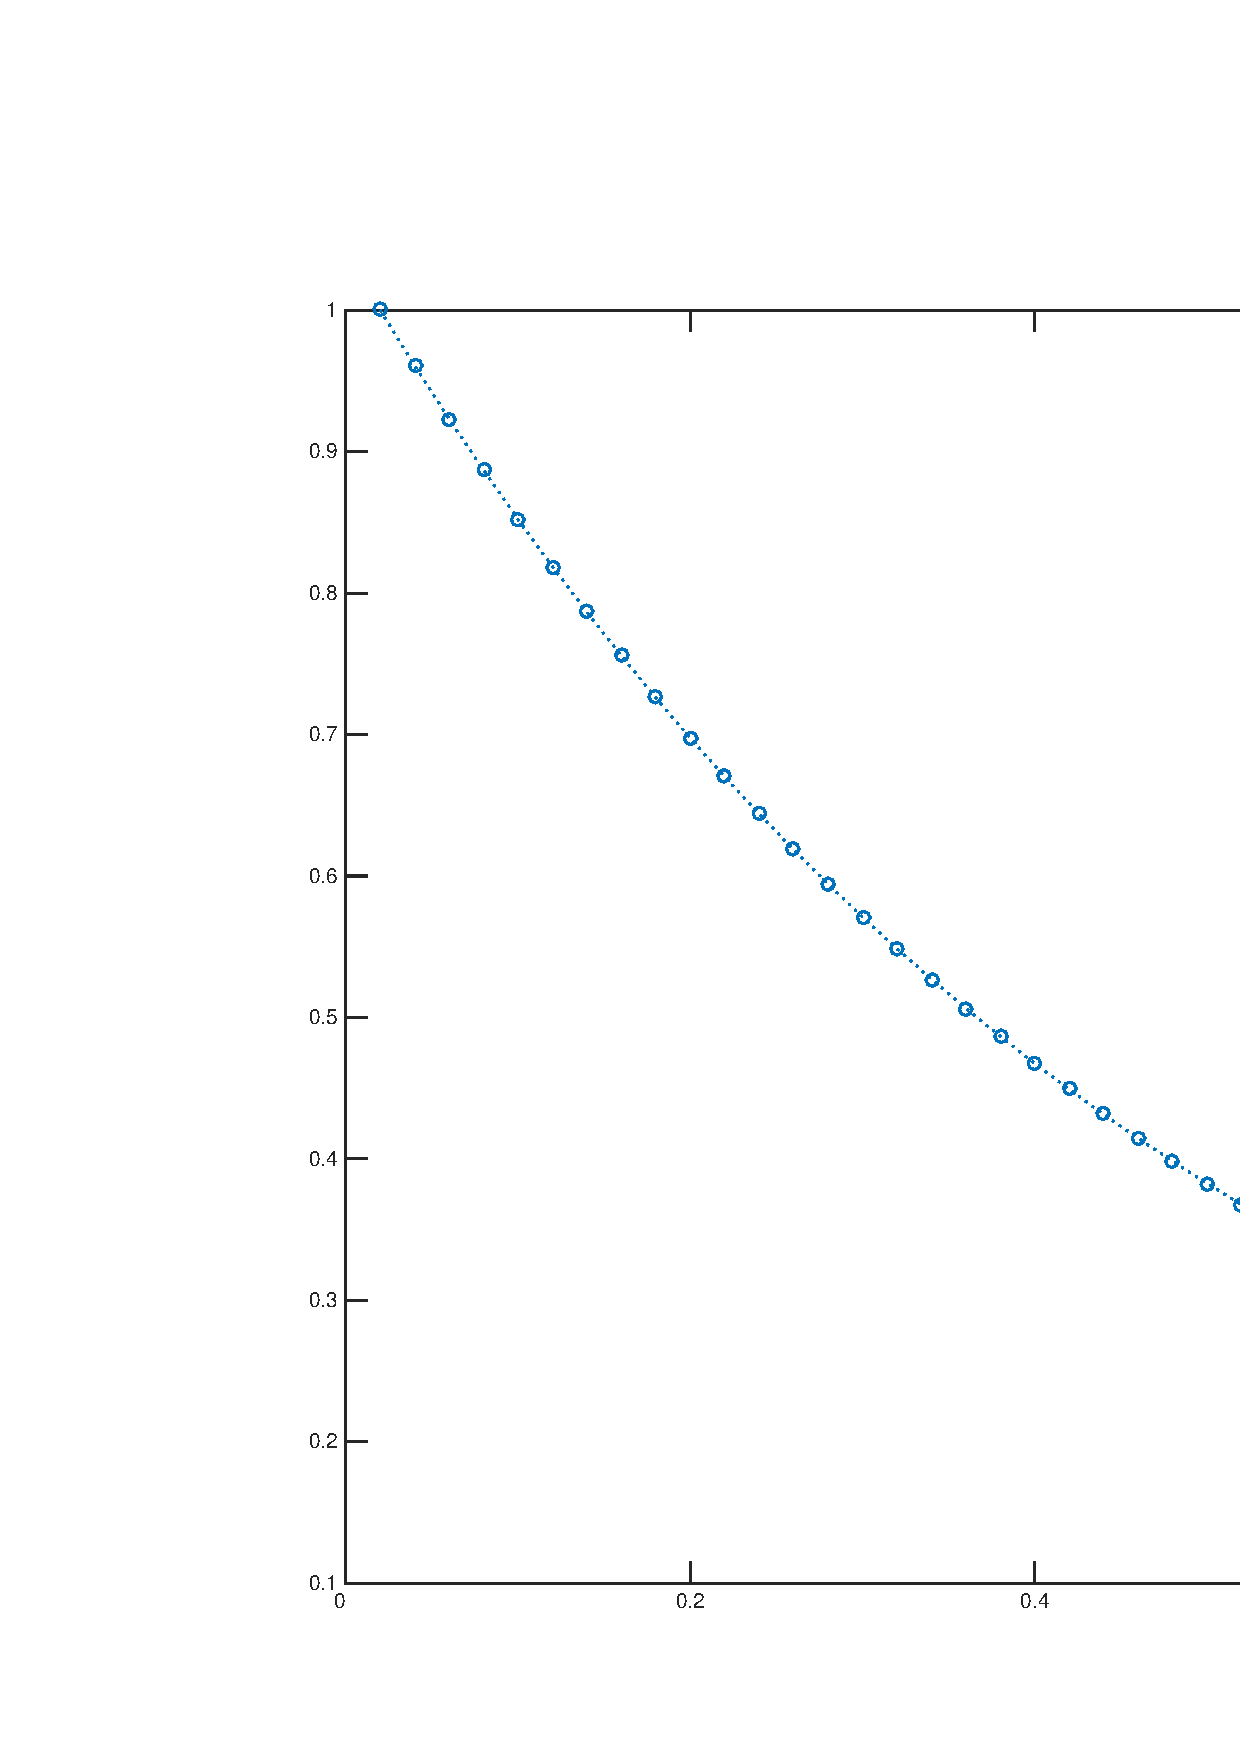
\includegraphics[width=8cm]{4.png}
\end{center}
\end{CJK*}
\end{document}
